\documentclass[tikz,border=5pt]{standalone}
\usepackage{tikz}
\usetikzlibrary{arrows.meta,positioning}
\begin{document}
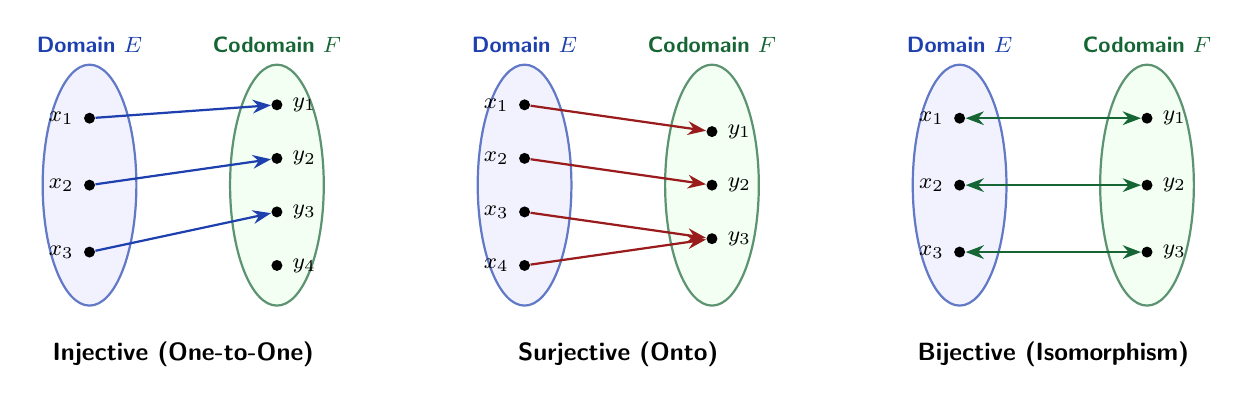
\begin{tikzpicture}[>=Stealth, scale=0.85]
  \definecolor{setblue}{HTML}{1E40AF}
  \definecolor{forestgreen}{HTML}{166534}
  \definecolor{accentcrimson}{HTML}{991B1B}

  % Injection
  \begin{scope}[shift={(0,0)}]
    \draw[thick, setblue!70, fill=blue!5] (-1,0) ellipse (0.7cm and 1.8cm);
    \draw[thick, forestgreen!70, fill=green!5] (1.8,0) ellipse (0.7cm and 1.8cm);
    \node[font=\sffamily\bfseries\footnotesize, setblue] at (-1, 2.1) {Domain $E$};
    \node[font=\sffamily\bfseries\footnotesize, forestgreen] at (1.8, 2.1) {Codomain $F$};
    \node[circle,fill=black,inner sep=1.4pt,label=left:{\footnotesize $x_1$}] (a1) at (-1, 1.0) {};
    \node[circle,fill=black,inner sep=1.4pt,label=left:{\footnotesize $x_2$}] (a2) at (-1, 0) {};
    \node[circle,fill=black,inner sep=1.4pt,label=left:{\footnotesize $x_3$}] (a3) at (-1, -1.0) {};
    \node[circle,fill=black,inner sep=1.4pt,label=right:{\footnotesize $y_1$}] (b1) at (1.8, 1.2) {};
    \node[circle,fill=black,inner sep=1.4pt,label=right:{\footnotesize $y_2$}] (b2) at (1.8, 0.4) {};
    \node[circle,fill=black,inner sep=1.4pt,label=right:{\footnotesize $y_3$}] (b3) at (1.8, -0.4) {};
    \node[circle,fill=black,inner sep=1.4pt,label=right:{\footnotesize $y_4$}] (b4) at (1.8, -1.2) {};
    \draw[->, thick, setblue] (a1) -- (b1);
    \draw[->, thick, setblue] (a2) -- (b2);
    \draw[->, thick, setblue] (a3) -- (b3);
    \node[below, font=\sffamily\small\bfseries] at (0.4,-2.2) {Injective (One-to-One)};
  \end{scope}

  % Surjection
  \begin{scope}[shift={(6.5,0)}]
    \draw[thick, setblue!70, fill=blue!5] (-1,0) ellipse (0.7cm and 1.8cm);
    \draw[thick, forestgreen!70, fill=green!5] (1.8,0) ellipse (0.7cm and 1.8cm);
    \node[font=\sffamily\bfseries\footnotesize, setblue] at (-1, 2.1) {Domain $E$};
    \node[font=\sffamily\bfseries\footnotesize, forestgreen] at (1.8, 2.1) {Codomain $F$};
    \node[circle,fill=black,inner sep=1.4pt,label=left:{\footnotesize $x_1$}] (c1) at (-1, 1.2) {};
    \node[circle,fill=black,inner sep=1.4pt,label=left:{\footnotesize $x_2$}] (c2) at (-1, 0.4) {};
    \node[circle,fill=black,inner sep=1.4pt,label=left:{\footnotesize $x_3$}] (c3) at (-1, -0.4) {};
    \node[circle,fill=black,inner sep=1.4pt,label=left:{\footnotesize $x_4$}] (c4) at (-1, -1.2) {};
    \node[circle,fill=black,inner sep=1.4pt,label=right:{\footnotesize $y_1$}] (d1) at (1.8, 0.8) {};
    \node[circle,fill=black,inner sep=1.4pt,label=right:{\footnotesize $y_2$}] (d2) at (1.8, 0) {};
    \node[circle,fill=black,inner sep=1.4pt,label=right:{\footnotesize $y_3$}] (d3) at (1.8, -0.8) {};
    \draw[->, thick, accentcrimson] (c1) -- (d1);
    \draw[->, thick, accentcrimson] (c2) -- (d2);
    \draw[->, thick, accentcrimson] (c3) -- (d3);
    \draw[->, thick, accentcrimson] (c4) -- (d3);
    \node[below, font=\sffamily\small\bfseries] at (0.4,-2.2) {Surjective (Onto)};
  \end{scope}

  % Bijection
  \begin{scope}[shift={(13.0,0)}]
    \draw[thick, setblue!70, fill=blue!5] (-1,0) ellipse (0.7cm and 1.8cm);
    \draw[thick, forestgreen!70, fill=green!5] (1.8,0) ellipse (0.7cm and 1.8cm);
    \node[font=\sffamily\bfseries\footnotesize, setblue] at (-1, 2.1) {Domain $E$};
    \node[font=\sffamily\bfseries\footnotesize, forestgreen] at (1.8, 2.1) {Codomain $F$};
    \node[circle,fill=black,inner sep=1.4pt,label=left:{\footnotesize $x_1$}] (e1) at (-1, 1.0) {};
    \node[circle,fill=black,inner sep=1.4pt,label=left:{\footnotesize $x_2$}] (e2) at (-1, 0) {};
    \node[circle,fill=black,inner sep=1.4pt,label=left:{\footnotesize $x_3$}] (e3) at (-1, -1.0) {};
    \node[circle,fill=black,inner sep=1.4pt,label=right:{\footnotesize $y_1$}] (f1) at (1.8, 1.0) {};
    \node[circle,fill=black,inner sep=1.4pt,label=right:{\footnotesize $y_2$}] (f2) at (1.8, 0) {};
    \node[circle,fill=black,inner sep=1.4pt,label=right:{\footnotesize $y_3$}] (f3) at (1.8, -1.0) {};
    \draw[<->, thick, forestgreen] (e1) -- (f1);
    \draw[<->, thick, forestgreen] (e2) -- (f2);
    \draw[<->, thick, forestgreen] (e3) -- (f3);
    \node[below, font=\sffamily\small\bfseries] at (0.4,-2.2) {Bijective (Isomorphism)};
  \end{scope}
\end{tikzpicture}
\end{document}